%Notes on a simple and eff net for small target detection, available on scihub: https://sci-hub.tw/10.1109/ACCESS.2019.2924960

In this article by Ju et al\., the authors try to address the issue of low small target detection performance in classical detection networks. The authors put forth 3 modifications to improve detection performance: first, a "dilated module" that helps to expand the recepetive field of convolutional layers without loss of resolution. Secondly, feature fusion is applied on the feature maps of different layers of the network . Finally, a passthrough layer, similar to the one described in You Only Look Twice\cite{yolt}, described in section \ref{yolt} and in ResNet\cite{resNet} is applied to get the finer-grained information from the earlier layers and the more semantic information coming out of the deeper layers.

The performance of the network is evaluated on the VEDAI\cite{vedai} dataset along with the DOTA\cite{dota} dataset, and obtains state of the art results, with FPS performance comparable to a tiny YOLOv3 network\cite{yolov3} but with average precision comparable to a "full size" YOLOv3 network.
\subsection{Proposed Modules}
\subsubsection{Dilated Modules}

\begin{figure}[h!]
\begin{subfigure}{.3\textwidth}
  \centering
  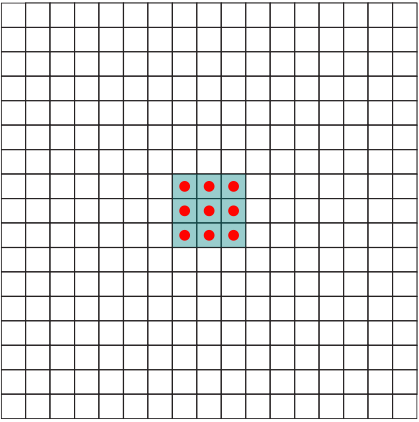
\includegraphics[width=.8\linewidth]{dilConvA.png}  
  \caption{1-Dilated Convolution}
\end{subfigure}
\begin{subfigure}{.3\textwidth}
  \centering
  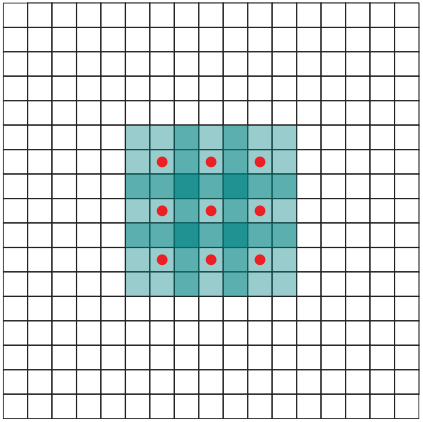
\includegraphics[width=.8\linewidth]{dilConvB.png}  
  \caption{2-Dilated Convolution}
\end{subfigure}
\begin{subfigure}{.3\textwidth}
  \centering
  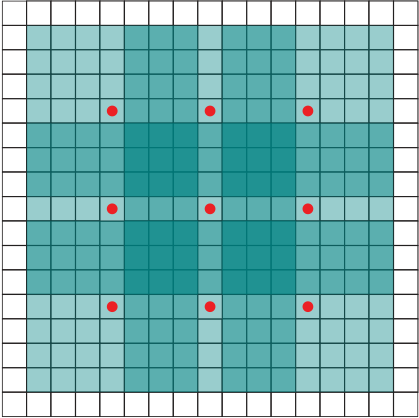
\includegraphics[width=.8\linewidth]{dilConvC.png}  
  \caption{4-Dilated Convolution}
\end{subfigure}
\caption{Dilated Convolution Example}
\label{fig:dilKernel}
\end{figure}

\textbf{Dilated convolution are used to expand the receptive field of the convolution operation without increasing the size of kernel or without reducing the size of the feature maps and losing information about small targets.} Figure \ref{fig:dilKernel} shows the dilatation of a convolution kernel and the impact on the receptive field. Dilated Convolution has been introduced by Yu and Koltum in "Multi-scale Context Aggregation by Dilated Convolutions"\cite{yu2015}.

Dilated modules are used to help to locate the small targets accurately and aggregate multi-scale contextual information. Dilated convolution is used as a basic element to build a dilated module. The module reuse features from earlier and deeper layer by concatenation. A $1 \times 1$ convolution is used to reduce the dimension of the module. 
\subsubsection{Passthrough module}

In a detection network, earlier layer contains more fine grained information which can be useful to detect and accurately determine the location of small objects. Usually this information is "lost" in the deeper layers. A passthrough layer with a stride of 2 is used to utilize those earlier features. The passthrough layer transform the feature map from a $2N \times 2N \times C$ to $N \times N \times 4C$. This passthrough layer is used to construct the passthrough module. This module merges features from earlier layers with the ones in the deeper layers. Again, a $1 \times 1$ convolution is used to reduce the dimension of the module.

\subsubsection{Feature Fusion}
Here, concatenation is used to merge features from earlier layers with ones coming from deeper layers. There are two different kind of fusion used in this paper. 

The first is concatenating the feature maps between different dilated modules. Since the dilated modules don't change the dimension of the feature maps, the merging can be directly done by concatenation.

The second kind is the passthrough layer. Since the feature maps undergoes downsampling, their dimensions changes. The paper propose to unify their dimension by using another passthrough layer and upsampling. 

\subsection{General Architecture} 
The proposed architecture is inspired by the tiny YOLOv3, but uses deeper layers along with dilated modules and feature fusion. $1 \times 1$ convolution are used to reduce the dimensions, which helps increase the speed and efficiency of the network.

\begin{figure}[h!]
	\centering
	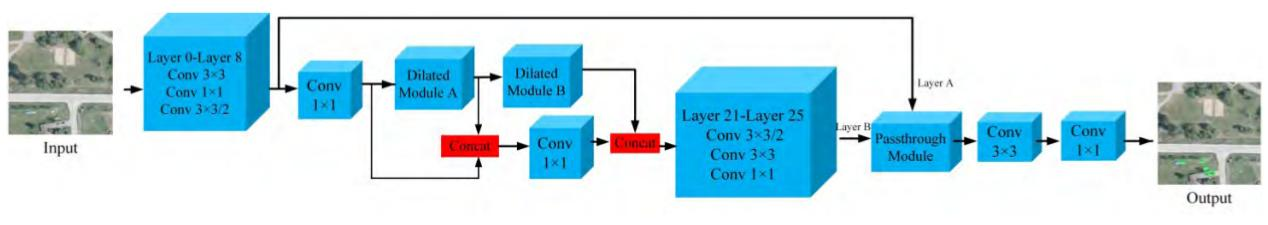
\includegraphics[width=\textwidth]{juArchi.jpg}
	\caption[General Architecture for the Simple and Efficient Network for Small Target Detection]{General Architecture}
	\label{fig:juGeneralArchi}
\end{figure}

Since the goal of the network is to detect small targets, large downsampling as the one used in YOLOv3 are not adequate. However, the number of downsampling layers affects the size of the receptive field, which in turns determines the amount of contextual information of small targets. Two dilated modules are used to expand the receptive field. The feature maps are downsampled twice and used as fine grained information and combine with feature maps that are downsampled thrice using a passthrough modules. 

The final layer provides the results of the prediction, which contains the location of the bounding box, and the class of the targets. The size of the last layer is $N = N_{boxes} \times (N_{classes} + 4 + 1)$ with 4 being the number of offsets for the bounding boxes, and 1 for the  "objectness" prediction. 

\subsection{Results}
The models were trained and tested on the VEDAI\cite{vedai} and DOTA datasets\cite{dota}. The authors notes that the targets in VEDAI are smaller than the ones in the DOTA datasets, but the quantity of targets in DOTA are higher than of VEDAI.

To obtain a good comparison between existing architectures and the proposed model, the author ran 4 experiments on both datasets, using YoloV2, Tiny YOLOv3, YOLOv3 and their own model. The same size of input ($512 \times 512$) was used on each model.

We should note that while YOLOv3 tends to obtain better scores in AP, the computing cost associated with running this algorithm in much higher, as it requires ten times more BFLOPs than the proposed model (see Table~\ref{tab:perfSimple}). This complexity is reflected in the number of Frames Per Seconds that is able to be computed. In short, it seems that the proposed method is able to obtain results similar, if slightly inferior than YOLOv3 but is much faster and has much less parameters than both YOLOv3 and tiny YOLOv3. 
\begin{table}[ht]
	\centering
	\begin{tabular}{@{}lllll@{}}
		\toprule
		Object Detection Algorithm & YOLOv2           & Tiny YOLOv3      & YOLOv3           & Proposed Model   \\ \midrule
		Input                      & $512 \times 512$ & $512 \times 512$ & $512 \times 512$ & $512 \times 512$ \\
		Model Size                 & 202.3M           & 34.7M            & 236.3M           & 2.8M             \\ \bottomrule
		FPS (Higher is better)     & 58.3             & \textbf{76.4}    & 14.7             & 75.4             \\
		BFLOPS (Lower is better)   & 44.417           & \textbf{8.243}   & 101.784          & 9.692            \\ 
		AP (Higher is better)      & 54.33            & 58.17            & \textbf{85.37}   & 80.16            \\ \bottomrule
	\end{tabular}
	\caption{Comparative results of FPS, BFLOPs and Model Size with all tested algorithms. BFLOPS refer to the number of billions of floating points operations needed to calculate the prediction.}
	\label{tab:perfSimple}
\end{table}
\clearpage

In short, this model combine the precision of YOLOv3 with the fast and efficient computation of the tiny model. 
